\begin{figure}[htbp]
  \centering
  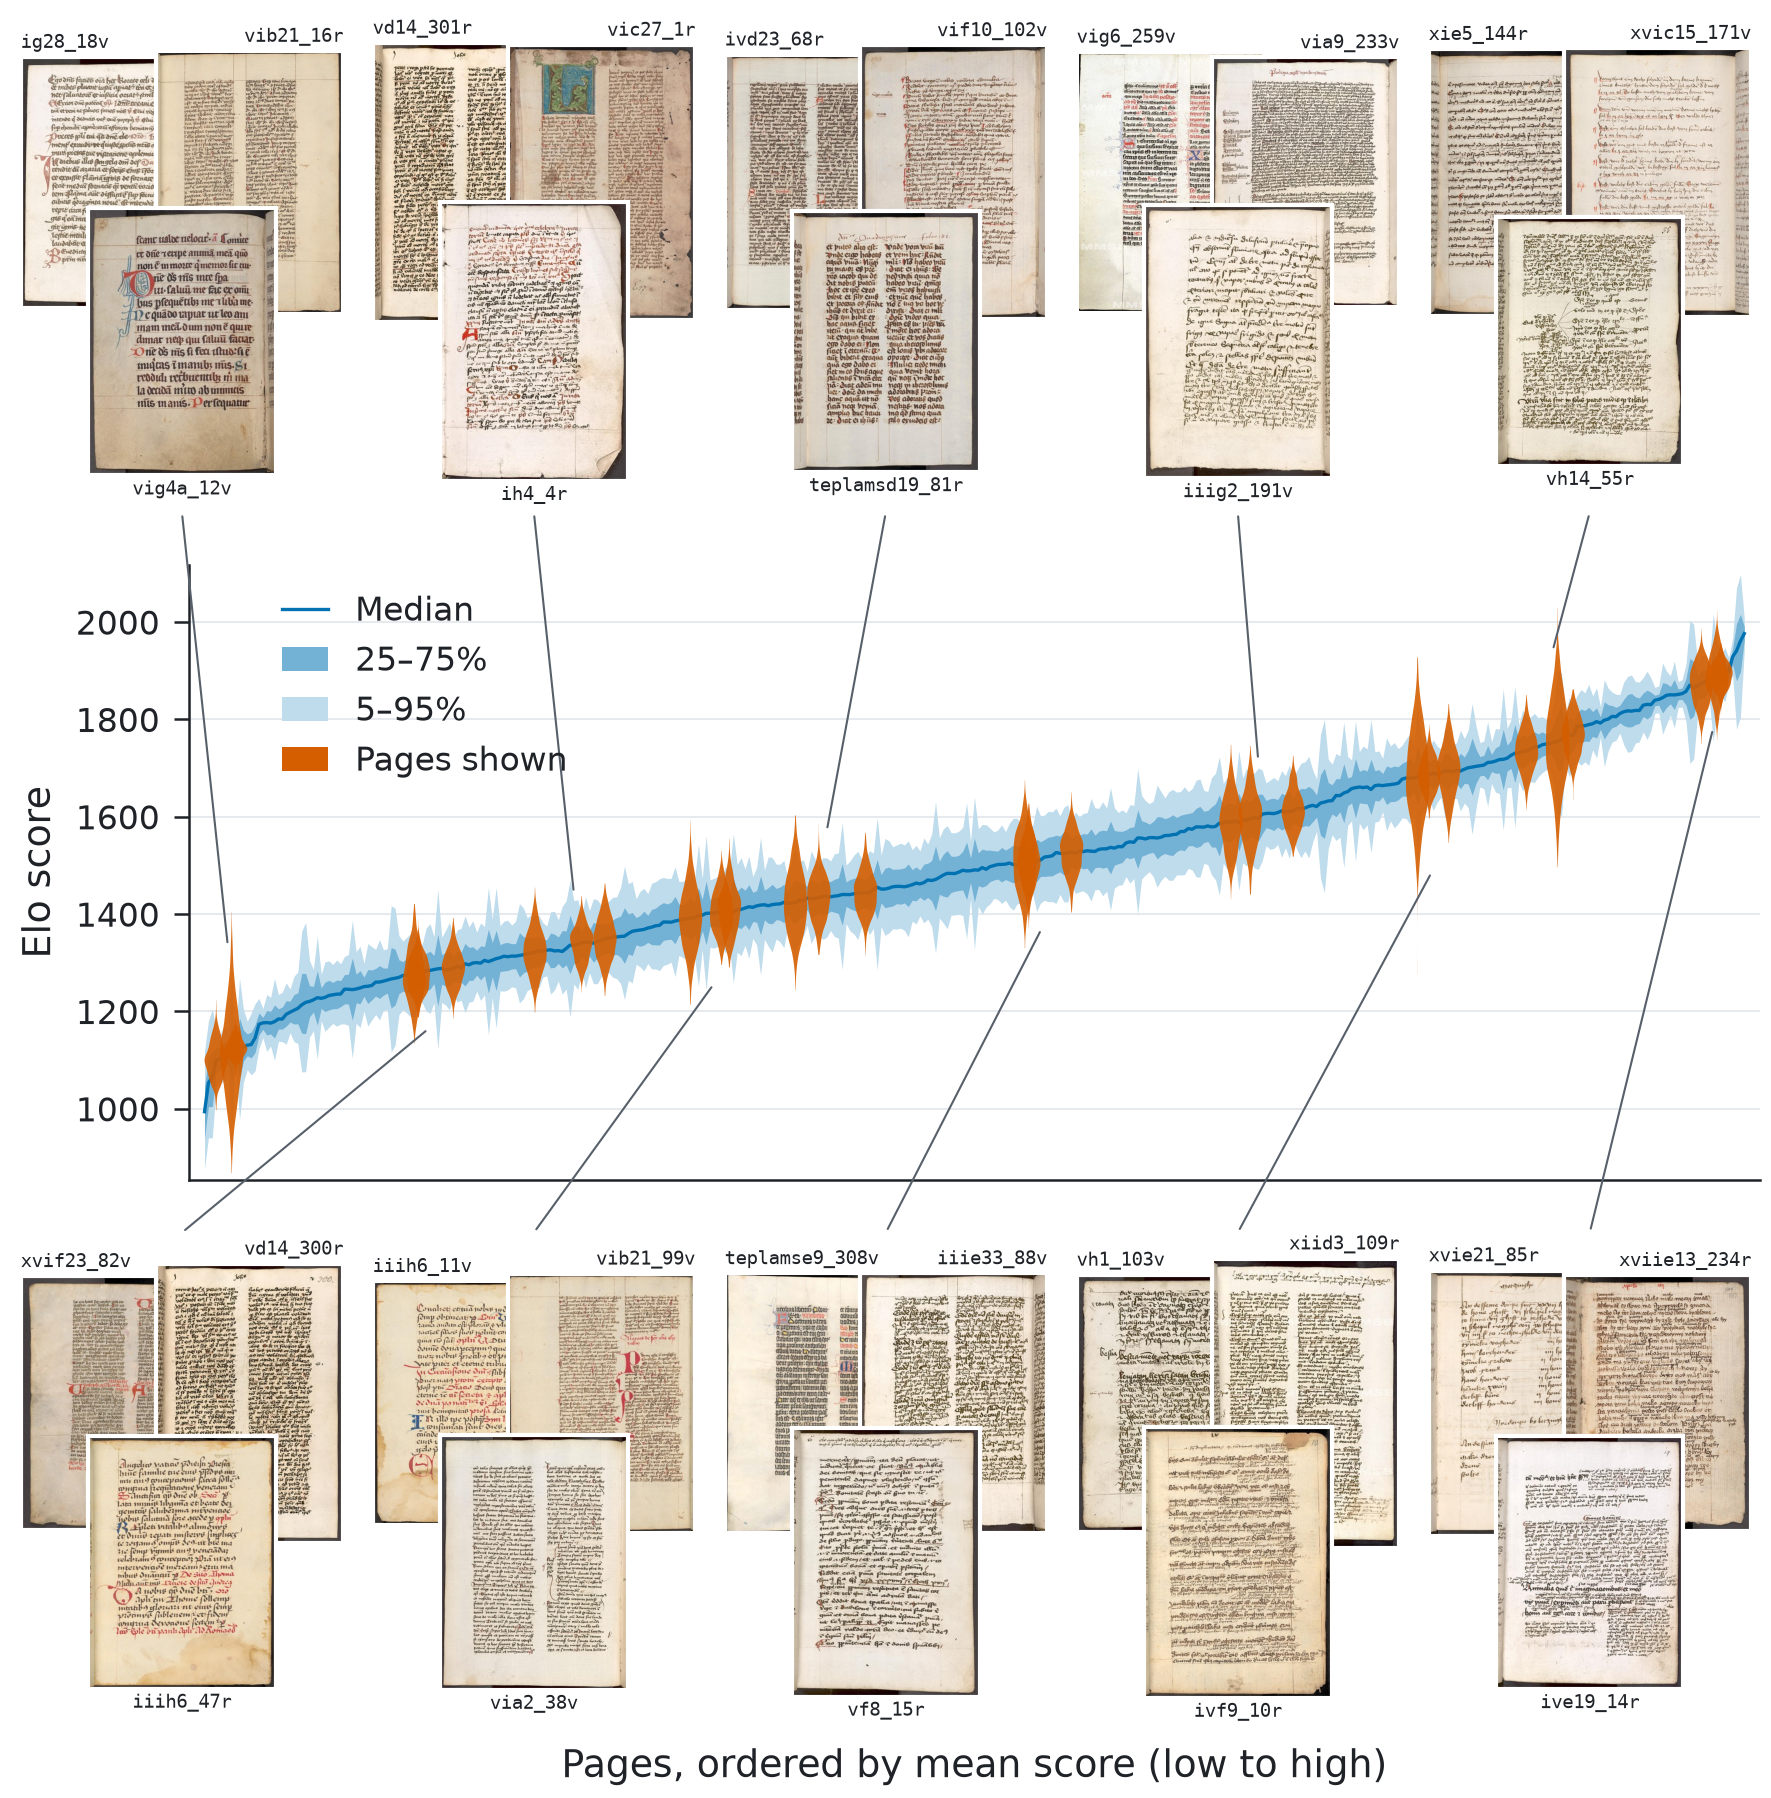
\includegraphics[width=15.00cm]{figures/elo_score_bands_trios.png}
  \caption{Visual complexity scores, three pages at each place. Computed as Elo scores over 1,000 random judgement order permutations. Images ordered by mean score from the lowest to the highest. Solid line shows the median. Dark and light blue bands indicate the middle half (25th to 75th percentiles) and the middle 90\% (5th to 95th percentiles), respectively. At each of the ten places, chosen near evenly spaced ranks, three pages whose mean scores lie within 31 points of each other are highlighted in vermillion and labelled with their ids. In front, the page typical of its score; behind it, two pages of common layouts from other manuscripts, as different from it and from each other as such pages get. A common layout has its text lines, columns, marginal zones, drop capitals, written and graphic shares and line spacing each within the 5th to 95th percentiles of the dataset's pages. Similar scores can belong to quite different layouts. Page images provided by Manuscriptorium (CC BY-NC 4.0).}
  \label{fig:elo_score_bands_trios}
\end{figure}
